\begin{figure}[t!]
    \centering
    % \begin{tabular}[c]{ccc}
    % \begin{subfigure}[c]{0.31\textwidth}
    %     \includegraphics[width=0.91\textwidth]{images/samples_by_artifact/30ms_coil_samples_1.eps}
    %     \caption{Coil-Combined SNR=7.5, drift aligned}
    %     % \vspace{3pt}
    % \end{subfigure}&
    % \begin{subfigure}[c]{0.31\textwidth}
    %     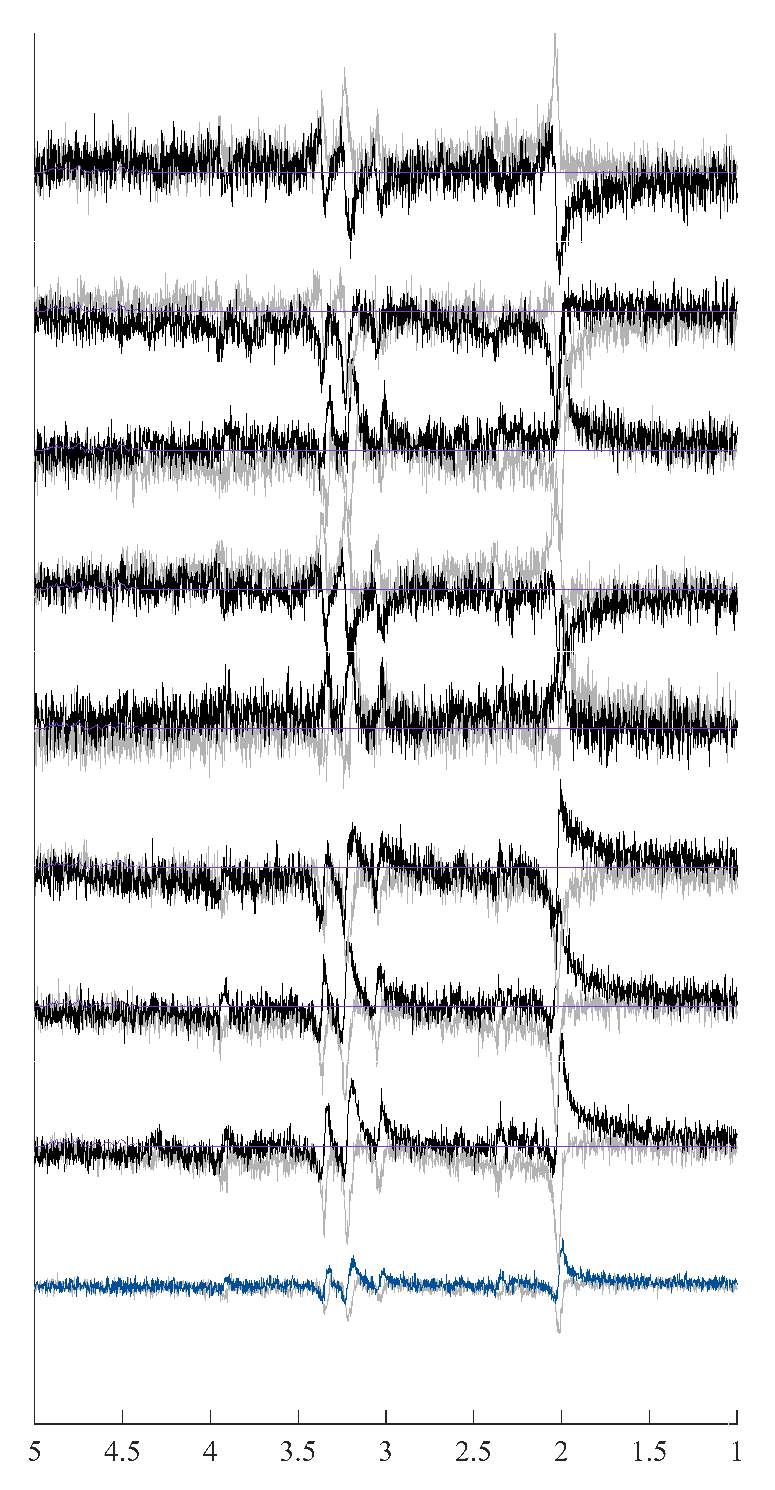
\includegraphics[width=0.91\textwidth]{images/samples_by_artifact/30ms_coil_samples_2.eps}
    %     \caption{Coil-Combined SNR=10, drift unaligned}
    %     % \hspace{1.5pt}
    %     % \vspace{3pt}
    % \end{subfigure}&
    % \begin{subfigure}[c]{0.31\textwidth}
    %     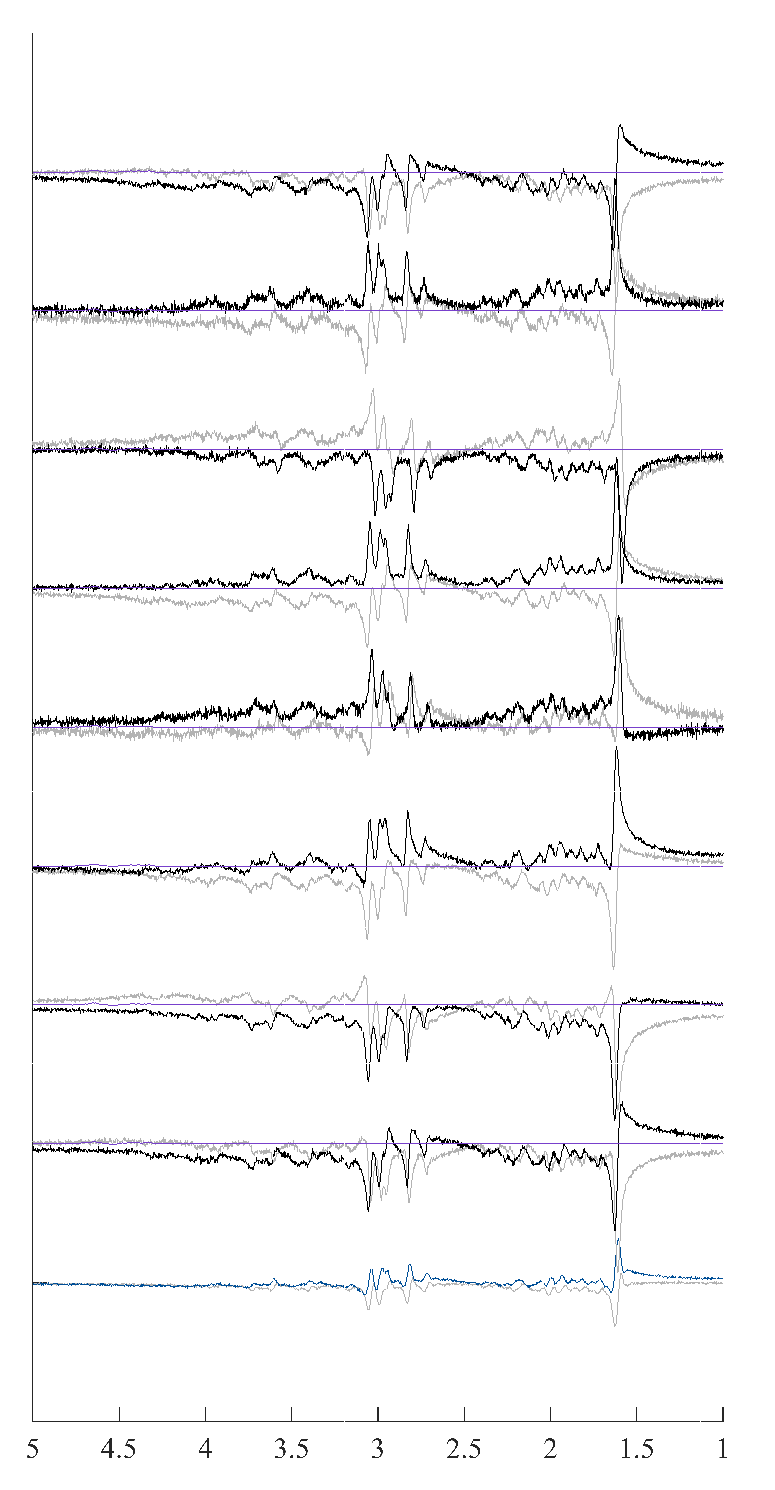
\includegraphics[width=0.91\textwidth]{images/samples_by_artifact/30ms_coil_samples_3.eps}
    %     \caption{Coil-Combined SNR=15, drift unaligned}
        
    %     % \hspace{3pt}
    %     % \vspace{3pt}
    % \end{subfigure}\\
    % \end{tabular}
    \includegraphics[width=0.9\textwidth,keepaspectratio]{images/compiled_figures/MRS_Sim_Figure_16_multicoil_transients_samples.png}
    \caption{These are examples of 8-channel simulated acquisitions. Their respective coil-combined spectra are shown at the bottom in blue. \textbf{(A)} shows low-SNR transients that have been phase- and frequency-drift aligned. \textbf{(B)} and \textbf{(C)} show transients with higher SNRs that have not been aligned, resulting in the coil-combined spectra having lower SNRs than otherwise expected.}
    \label{fig:30ms samples coils}
\end{figure}

